\section{The Vapnik-Chervanenkis (VC) dimension}

\mode<presentation>{
\begin{frame} 
    \begin{center} \huge
        \secname
    \end{center}
\end{frame}
}

\begin{frame}\frametitle{Shattering p points}

\question{Can a perceptron classify any 3 points in 2D?}\\

\textbf{see blackboard...}


\question{Can a perceptron classify any 4 points in 2D?}\\


\textbf{see blackboard...}


\pause

\begin{enumerate}
\item Generate a dataset of $p$ points in $N$ dimensions and place them in some arrangement.
\item Decide on a model class $\Lambda$ (e.g. connectionist neuron)
\item For each possible binary label configuration (total: $2^p$) $\{y_T^{(\alpha)}\}_{\alpha=1}^p$ do
	\begin{itemize}
	\item[] Train the paramters $\vec w$ of a model from the set $\Lambda$.
	\item[] Generate binary predictions $\{y^{(\alpha)}(\vec x^{(\alpha)}; \vec w)\}_{\alpha=1}^p$
	\item[] Measure the error $E^T_{[\vec w]}$
	\item[] If $E^T_{[\vec w]} = 0$ keep the model, otherwise, discard it. 
	\end{itemize}
\item Count how many models you kept.\\
\item[] If you were able to keep a model with $E^T_{[\vec w]} = 0$ for each of the $2^p$ possible label configurations,\\
then the model class $\Lambda$ with that number of tunable parameters in $\vec w$ \emph{shatters} a dataset of $p$ points in $N$ dimensions.
\end{enumerate}

\textbf{Important}:\\

Shattering requires finding only a single arrangment of the $p$ points for which the model can be fitted to all $2^p$ label configurations.

\mode<article>{
It does not have to be able to for all possible arrangements (placements) of the $p$ points.
If there exists at least \textbf{one} dataset for which it can perfectly predict all label configurations, then the model shatters this.
}
\end{frame}

\begin{frame}\frametitle{\secname}

$\dvc$ is not actually a dimension but a \emph{capacity measure} 
of a model class that is parameterized by $\vec w$.

\underline{Definition}:\\

$\dvc :=$ \underline{maximal number of data points $p$} that a model can \emph{shatter}.

In other words: $\dvc$ is \underline{maximal number of data points $p$} for which \emph{all} possible label configurations $\{y_{T}^{(\alpha)} \in \{-1,1\}\}_{\alpha=1}^{p}$ can be perfectly trained (i.e. $E^{T}_{[\vec w]} = R_{\text{emp}[\vec w]} = 0$) by tuning the model parameters $\vec w$.
If (at least) one dataset $\{(\vec x^{(\alpha)}, y_{T}^{(\alpha)})\}_{\alpha=1}^{p}$ with $p$ points exists such that the model can be tuned to perfectly classify any label configuration for that dataset, then the $\dvc$ for this model class is $p$.


\question{What was the $\dvc$ for our model in the previous example?}

\end{frame}

\begin{frame}

\underline{Examples}:

\begin{itemize}
\item $\dvc^{\text{perceptron}} = N+1 = $\# params.
\item $\dvc^{\text{MLP}} = \mathcal{O}$(\# params.$^{2}$)
\item $\dvc^{\text{sinusoid}} = \infty$
\end{itemize}
    
\end{frame}

\subsection{Results statistical learning theory}

\begin{frame}\frametitle{Results statistical learning theory}
		\begin{itemize}
			\item Learnability - Convergence of Empirical risk minimization is guaranteed (cf. \sectionref{sec:convergence_erm})
			\item formulation of conditions under which ERM works
			\item bounds describing \textbf{generalization ability} of ERM 
			\item inductive inference for \textbf{small sample size}s 
				based on these bounds
			\item methods for implementing this new type 
				of inference ($\rightarrow$ {SVMs})
		\end{itemize}
\end{frame}

\subsubsection{Learnability - Convergence of Empirical risk minimization (ERM)}

\begin{frame}\frametitle{\subsecname}\label{sec:convergence_erm}
			
			Convergence of Empirical risk minimization is guaranteed:
			
			For a model class with \emph{finite} $\dvc$, the empirical training error will converge to the generalization error
			with more data. That is:
			\begin{equation}
				\lim_{p \to \infty}
						E^T_{[\vec w]} = E^G_{[\vec w]}
			\end{equation}
			
			The requirement is that $\dvc$ is \emph{finite}.
			
			\mode<article>{The training error converges to the generalization error.
			}
			In terms of risk, this would be:
			
			\begin{equation}
				\lim_{p \to \infty} 
					R_{\text{emp}[\vec w]} = R_{[\vec w]}
			\end{equation}
			
			Another way to look at this is to measure the difference between $R_{(\vec w_p)}$ and $R_{(\vec w_0)}$, where
			\begin{itemize}
			\item $R_{(\vec w_p)}$ is the empirical risk obtained from training the model using a finite set with $p$ points, and
			\item $R_{(\vec w_0)}$ risk obtained from training the model with inifinite many points (Don't treat the $_0$ as zero points but rather ``minimal'').
			\end{itemize}
			
			And this difference becoming smaller and smaller as we feed more points into the model. That is:
			\begin{equation}
				\lim_{p \to \infty} P\bigg\{ 
					{
						\Big|R_{[\vec w_p]} - R_{[\vec w_0]}\Big| 
					}
				\geq \eta \bigg\}\;\;=\;\; 0 \,, \quad \forall \eta > 0
			\end{equation}
			
			Understanding what $P\bigg\{ 
					{
						\Big|R_{(\vec w_p)} - R_{(\vec w_0)}\Big| 
					}
				\geq \eta \bigg\}$ represents:
			
			\begin{itemize}
			\item We expect the model trained on $p$ points to accumulate some error $R_{(\vec w_p)}$.
			\item Training the model with a different set of $p$ points may yield a different value for $R_{(\vec w_p)}$.
			\item Training many models with $p$ will yield many values for $R_{(\vec w_p)}$.
			\item Measuring the absolute difference between every $R_{(\vec w_p)}$ we obtained and $R_{(\vec w_0)}$ will lead to ``difference values'' that follow some distribution $P\bigg\{ 
					{
						\Big|R_{[\vec w_p]} - R_{[\vec w_0]}\Big| 
					}
				\geq \eta \bigg\}$
			\item We measure the probability of the absolute difference exceeding some value $\eta$:
			\begin{equation}
			P\bigg\{ 
					{
						\Big|R_{[\vec w_p]} - R_{[\vec w_0]}\Big| 
					}
				\geq \eta \bigg\}\,, \quad \forall \eta > 0
			\end{equation}
			This is the same asking how often does traning with $p$ points yield a difference in risk above some value.
			\item Now repeat tranining these models but using a larger value for $p$.\\
			What the theory tells you is that as you increase $p$ and keeping $\eta$ fixed:
			\begin{itemize}
			\item The $R_{[\vec w_p]}$ of the models will improve and get smaller.
			\item The absolute differences $\Big|R_{[\vec w_p]} - R_{[\vec w_0]}\Big|$ will become smaller and smaller,
			\item The distribution of these differences will shift below $\eta$ (i.e. to the left of $\eta$)
			\item Less and less models will score differences $\ge \eta$
			\item Eventually, for some large $p$, the $R_{[\vec w_p]}$ of the models will be so good that the probability of finding a model that has a risk difference of $\eta$ or higher (worse performance) will vanish. And this is what \eqref{eq:risktozero} describes:
			\end{itemize}
			
			\end{itemize}
			
			\begin{equation}
				\lim_{p \to \infty} P\bigg\{ 
					{
						\Big|R_{(\vec w_p)} - R_{(\vec w_0)}\Big| 
					}
				\geq \eta \bigg\}\;\;=\;\; 0 \,, \quad \forall \eta > 0
				\label{eq:risktozero}
			\end{equation}
			
			\textbf{But} Our dataset is never going to be inifinitley large. Therefore a more realistic formulation for the convergence of ERM would be:
			
			
\end{frame}


\begin{frame}\frametitle{The solution to learning problem 2} 
	\begin{center}
		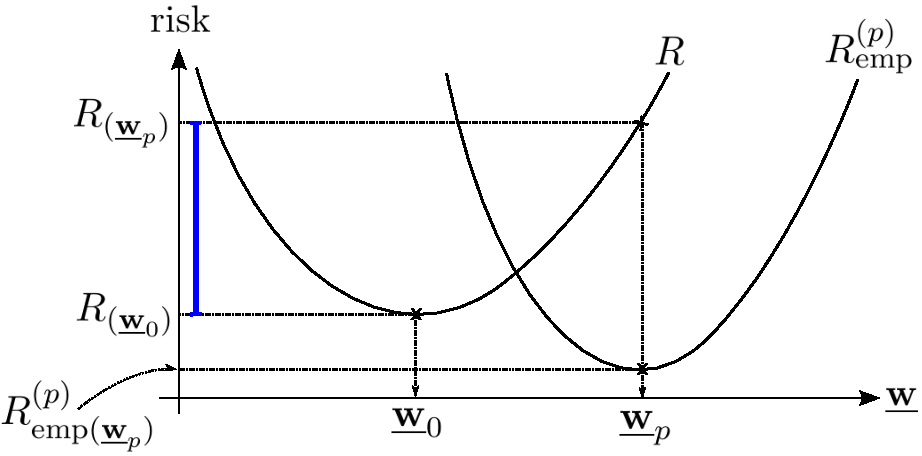
\includegraphics[width=9cm]{img/section2_fig1_question1}
	\end{center}
	\begin{enumerate}\setcounter{enumi}{1}
		\item {\textbf finite samples:} deviation from the optimal model
			\vspace{-2mm}
			$$
				P\bigg\{ {%\color{question1} 
				\Big| R_{(\vec w_p)} - R_{(\vec w_0)} \Big| }
					> \Big(\smallfrac{G^\Lambda_{(2p)} 
						- \ln \frac{\epsilon}{8}}{p} \Big)^\frac{1}{2}
					+ \Big(-\smallfrac{\ln \frac{\epsilon}{2}}{2p} 
						\Big)^\frac{1}{2} + \smallfrac{1}{p}
				\bigg\} < \epsilon
			$$
			\vspace{-4mm}
			\iitem{ finite $\dvc$: increased sample size $p$ 
				$\Rightarrow$ reduction of the bound}
	\end{enumerate}
\end{frame}

\begin{frame}\frametitle{The solution to learning problem 3} 
	\begin{center}
		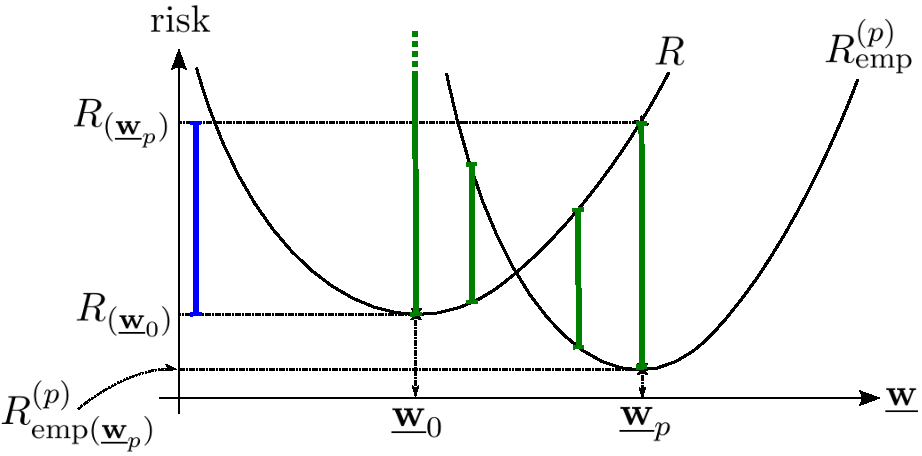
\includegraphics[width=9cm]{img/section2_fig1_question2_lessw}
	\end{center}
	\begin{enumerate}\setcounter{enumi}{2}
		\item {\textbf finite samples:} bound on the generalization error
			\vspace{-2mm}
			$$
				P\bigg\{ \sup\limits_{\vec w \in \Lambda}
					{%\color{question2} 
						\Big|R_{(\vec w)} - R^{(p)}_{\text{emp}(\vec w)}\Big| 
					} > \eta
				\bigg\} < 4 \exp\Big( G^\Lambda_{(2p)} 
					- p \big( \eta - \smallfrac{1}{p} \big)^2 \Big)
			$$
			\vspace{-4mm}
			\iitem{ bound non-trivial only if $G^\Lambda_{(2p)}$ 
				is sub-linear in $p$					
				\hfill {\scriptsize(see blackboard)}}
	\end{enumerate}
\end{frame}
